\begin{activity} \label{A:2.8.2}  
In this activity, we reason graphically from the following figure to evaluate limits of ratios of functions about which some information is known.
\begin{figure}[h]
\begin{center}
\scalebox{0.9}{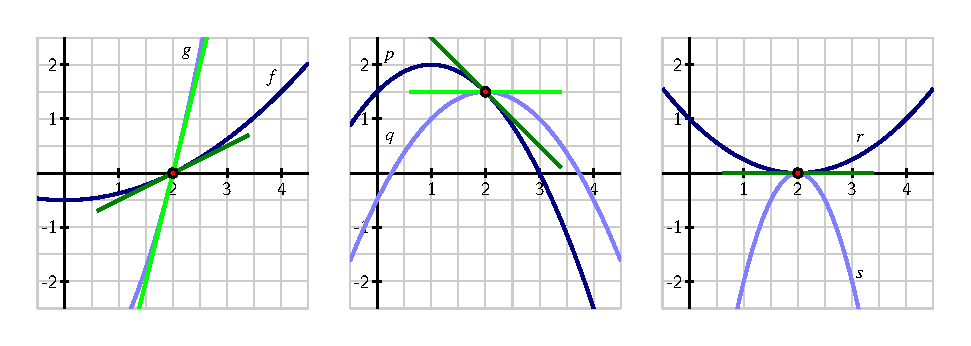
\includegraphics{figures/2_8_Act2.eps}}
\caption{Three graphs referenced in the questions of Activity~\ref{A:2.8.2}.} \label{F:2.8.Act2}
\end{center}
\end{figure}
\ba
	\item Use the left-hand graph to determine the values of $f(2)$, $f'(2)$, $g(2)$, and $g'(2)$.  Then, evaluate 
	$$\lim_{x \to 2} \frac{f(x)}{g(x)}.$$
	\item Use the middle graph to find $p(2)$, $p'(2)$, $q(2)$, and $q'(2)$.  Then, determine the value of
	$$\lim_{x \to 2} \frac{p(x)}{q(x)}.$$
	\item Use the right-hand graph to compute $r(2)$, $r'(2)$, $s(2)$, $s'(2)$.  Explain why you cannot determine the exact value of 
	$$\lim_{x \to 2} \frac{r(x)}{s(x)}$$
	without further information being provided, but that you can determine the sign of $\lim_{x \to 2} \frac{r(x)}{s(x)}$.  In addition, state what the sign of the limit will be, with justification.
\ea
\end{activity}
\begin{smallhint}
\ba
	\item Don't forget that $f'(a)$ measures the slope of the tangent line to $y = f(x)$ at the point $(a,f(a))$.
	\item Do the functions $p$ and $q$ meet the criteria of L'Hopital's Rule?
	\item Remember that L'Hopital's Rule can be applied more than once to a particular limit.
\ea
\end{smallhint}
\begin{bighint}
\ba
	\item Don't forget that $f'(a)$ measures the slope of the tangent line to $y = f(x)$ at the point $(a,f(a))$.  Think about whether or not L'Hopital's Rule applies to the limit under consideration.
	\item Do the functions $p$ and $q$ meet the criteria of L'Hopital's Rule?  If not, what are your options for evaluating the limit?
	\item Remember that L'Hopital's Rule can be applied more than once to a particular limit and that the sign of $f''(a)$ is connected to to the concavity of the graph of $f$ at the value $x = a$.
\ea
\end{bighint}
\begin{activitySolution}
\ba
	\item From the given graph, we observe that $f(2) = 0$, $f'(2) = \frac{1}{2}$, $g(2)=0$, and $g'(2) = 4$.  By L'Hopital's Rule, 
	$$\lim_{x \to 2} \frac{f(x)}{g(x)} = \frac{f'(2)}{g'(2)} = \frac{\frac{1}{2}}{4} = \frac{1}{8}.$$
	\item The given graph tells us that $p(2) = 1.5$, $p'(2)=-1$, $q(2)=1.5$, and $q'(2)=0$.  Note well that the given limit,
	$$\lim_{x \to 2} \frac{p(x)}{q(x)},$$
	is not indeterminate, and thus L'Hopital's Rule does not apply.  Rather, since $p(x) \to 1.5$ and $q(x) \to 1.5$ as $x \to 2$, we have that 
	$$\lim_{x \to 2} \frac{p(x)}{q(x)} = \frac{p(2)}{q(2)} = \frac{1.5}{1.5} = 1.$$
	\item From the third graph,  $r(2)=0$, $r'(2)=0$, $s(2)=0$, $s'(2)=0$.  By L'Hopital's Rule,
	$$\lim_{x \to 2} \frac{r(x)}{s(x)} = \lim_{x \to 2} \frac{r'(x)}{s'(x)},$$
	but this limit is still indeterminate, so by L'Hopital's Rule again,
	$$\lim_{x \to 2} \frac{r(x)}{s(x)} = \lim_{x \to 2} \frac{r''(x)}{s''(x)} = \frac{r''(2)}{s''(2)},$$
provided that $s''(2) \ne 0$.  Since we do not know the values of $r''(2)$ and $s''(2)$, we can't determine the actual value of the limit, but from the graph it appears that $r''(2) > 0$ (since $r$ is concave up) and that $s''(2) < 0$ (because $s$ is concave down), and therefore
	$$\lim_{x \to 2} \frac{r(x)}{s(x)} < 0.$$
\ea
\end{activitySolution}
\aftera